\documentclass[11pt]{article}
\usepackage[T1]{fontenc}
\usepackage{amsmath,amssymb,amsthm,mathtools}
\usepackage{graphicx}
\usepackage[margin=0.88in]{geometry}
\usepackage{microtype}
\usepackage[hidelinks]{hyperref}

\newtheorem{theorem}{Theorem}
\newtheorem{remark}[theorem]{Remark}
\newcommand{\C}{\mathbb C}
\newcommand{\N}{\mathbb N}

\title{A six-vector counterexample to the proposed $\ell_p$ plank theorem\\
\large A negative answer to Question 6.13 of arXiv:1209.1462}
\author{Autonomous proof packet --- agent\_lane\_12}
\date{11 August 2026}

\begin{document}
\maketitle

\begin{abstract}
Question 6.13 asks for a simultaneous lower-bound vector in the dual of
complex $\ell_p$ whenever the prescribed lower bounds have unit
$\ell_{\min\{2,q\}}$ norm.  We give a counterexample at the endpoint
$p=1$, $q=\infty$.  Two coordinate functionals and four diagonal
functionals in $\ell_1^2$, all with threshold $2/5$, already exclude every
point of the unit ball of $\ell_\infty$.  Their squared thresholds total
only $24/25$.  A strictly positive geometric tail uses the remaining
$1/25$, producing exactly the infinite sequences required in the question.
The proof is an elementary four-point covering of the complex projective
line, with strict rational margins.
\end{abstract}

\section{The source question}

The source is S.~Shkarin, \emph{Non-sequential weak supercyclicity and
hypercyclicity}, arXiv:1209.1462~\cite{source}.  Question 6.13 on PDF page 33
asks whether, for conjugate $p,q$, $r=\min\{2,q\}$, unit vectors
$x_n\in\ell_p$, and positive $s_n$ with $\sum s_n^r=1$, there must be a unit
$y\in\ell_q$ satisfying $|\langle x_n,y\rangle|\ge s_n$ for every $n$.

\begin{center}
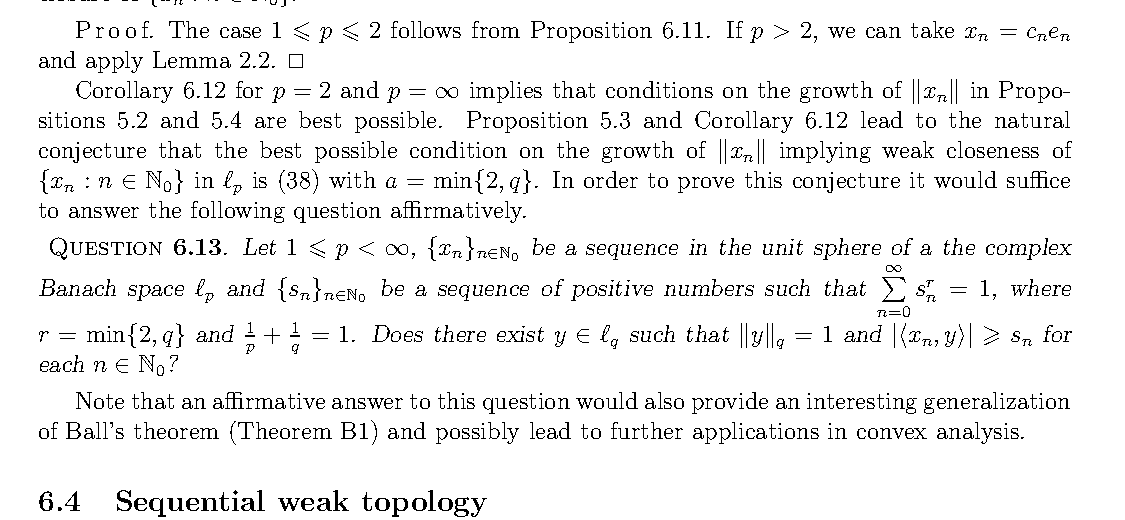
\includegraphics[width=0.97\textwidth]{figures/question_6_13_crop.png}
\end{center}

We use the bilinear dual pairing
$\langle x,y\rangle=\sum_jx(j)y(j)$.  The same construction works for the
conjugate convention because the set of fourth roots of unity is closed
under conjugation.

\section{Counterexample}

\begin{theorem}\label{thm:main}
The answer to Question 6.13 is negative.  In fact, for $p=1$, $q=\infty$
there are sequences $(x_n)_{n\ge0}$ in the unit sphere of complex $\ell_1$
and positive numbers $(s_n)_{n\ge0}$ such that
\[
 \sum_{n=0}^{\infty}s_n^2=1,
\]
but no $y\in\ell_\infty$ of norm one satisfies
$|\langle x_n,y\rangle|\ge s_n$ for every $n$.
\end{theorem}

\begin{proof}
Let $e_1,e_2$ be the first two coordinate vectors and put
\[
 \Omega=\{1,-1,i,-i\}.
\]
Take as the first six vectors
\[
 x_0=e_1,\qquad x_1=e_2,\qquad
 \{x_2,x_3,x_4,x_5\}
 =\left\{\frac{e_1-\overline\omega e_2}{2}:\omega\in\Omega\right\}.
 \tag{1}
\]
Every vector in (1) has $\ell_1$ norm one.  Set
\[
 s_0=\cdots=s_5=\frac25.                                      \tag{2}
\]

We first show that the six inequalities from (1)--(2) already have no
simultaneous solution in the closed unit ball of $\ell_\infty$.  Let
$\|y\|_\infty\le1$.  If either $|y(1)|<2/5$ or $|y(2)|<2/5$, one of the two
coordinate inequalities fails.  We may therefore assume both coordinate
moduli are at least $2/5$.

Let $m=\max\{|y(1)|,|y(2)|\}\le1$.  Divide the first two coordinates by a
common unimodular scalar.  Using the larger coordinate as the projective
denominator, their ratio has the form $z=\rho e^{i\theta}$ with
\[
 \frac25\le\rho\le1.                                         \tag{3}
\]
Choose $\omega\in\Omega$ whose argument differs from $\theta$ by at most
$\pi/4$.  Whether the first or second coordinate is the denominator, one of
the four diagonal correlations has modulus
\[
 \frac m2|z-\omega|.
\]
Since $\cos(\theta-\arg\omega)\ge1/\sqrt2$,
\[
 |z-\omega|^2
 \le 1+\rho^2-\sqrt2\,\rho.                                 \tag{4}
\]
The right side of (4) is convex in $\rho$, so its maximum on the interval
in (3) occurs at an endpoint.  The two endpoint values satisfy
\[
 2-\sqrt2<\frac{16}{25},
 \qquad
 \frac{29}{25}-\frac{2\sqrt2}{5}<\frac{16}{25}.              \tag{5}
\]
Indeed, the inequalities in (5) reduce respectively to
$2>(34/25)^2$ and $2>(13/10)^2$.  It follows that
$|z-\omega|<4/5$, and therefore the selected diagonal correlation is
strictly smaller than
\[
 \frac m2\frac45\le\frac25.
\]
Thus at least one of the first six required inequalities always fails.

It remains only to make the sequence of thresholds infinite, strictly
positive, and exactly normalized.  For $k\ge1$, define
\[
 x_{5+k}=e_1,
 \qquad
 s_{5+k}=\frac{\sqrt3}{5}\,2^{-k}.                           \tag{6}
\]
All the $x_n$ are unit vectors of $\ell_1$ and all $s_n$ are positive.
Moreover,
\[
 \sum_{n=0}^{\infty}s_n^2
 =6\left(\frac25\right)^2
   +\frac3{25}\sum_{k=1}^{\infty}4^{-k}
 =\frac{24}{25}+\frac1{25}=1.
\]
The tail cannot restore a simultaneous solution already excluded by the
first six constraints.  Zero-padding the vectors embeds the construction
from $\C^2$ into the source's infinite-dimensional sequence spaces.
\end{proof}

\section{Geometry, checks, and scope}

The two coordinate functionals say that a candidate must lie in the
projective annulus where the smaller of its first two coordinates is not too
small.  The other four functionals have zero directions at the fourth roots
of unity.  Every point of that annulus is within Euclidean distance $4/5$
of one of those roots.  The factor $1/2$ in the $\ell_1$ normalization then
makes the corresponding correlation smaller than $2/5$.  The endpoint
checks in (5) are strict, so equality cases and nonattainment of the
$\ell_\infty$ norm cause no difficulty.

The companion script \texttt{code/verify\_counterexample.py} checks the two
exact rational margins, the norm and budget identities, and a dense
diagnostic grid for (4).  The proof itself is exact and does not depend on
the numerical grid.

This gives a full negative answer to the universal statement of Question
6.13.  It does \emph{not} disprove the separate weak-closedness conjecture
that motivated the question: the source says only that an affirmative answer
to Question 6.13 would suffice for that conjecture.

Bounded novelty checks on 11 August 2026 covered the run's cheap indexes and
arXiv/web searches by exact title, arXiv id, question number, and the
$\ell_p$ plank formulation.  They found the source and later plank surveys,
but no cited resolution of Question 6.13 or this six-vector example.  This
is a search report, not a priority claim.

\paragraph{Human-review recommendation.}
Accept as a candidate full counterexample.  The only substantive checks are
the four-root covering estimate (4)--(5) and the positive-tail normalization;
both are elementary and strict.

\begin{thebibliography}{9}
\bibitem{source}
S.~Shkarin,
\emph{Non-sequential weak supercyclicity and hypercyclicity},
arXiv:1209.1462 (2012), Question 6.13.
\end{thebibliography}

\end{document}
